

Las gráficas mostradas a continuación estan basadas en los archivos de salida generados por el programa principal, los cuales fueron analizados y convertidos en gráficos mediante \textbf{generateImages.py}. Los mismos datos se encuentran disponibles LINK[aquí], donde se puede ver sus versiones adaptadas a la lectura y su contraparte de datos brutos 
pensados para ser procesados por el script de gráficos.

Si el lector quiere consultar los resultados de cada uno de estos casos de pruebas, los archivos con esa información se encuentran 
LINK[aqui], donde puede comparar las respuestas entregadas por cada uno de los algoritmos.

De ahora en adelante, nos referiremos a los algoritmos como DP (Dynamic Programming) y BF (Brute Force).

\begin{figure}[H]
    \centering
    \begin{minipage}[t]{0.5\textwidth}
        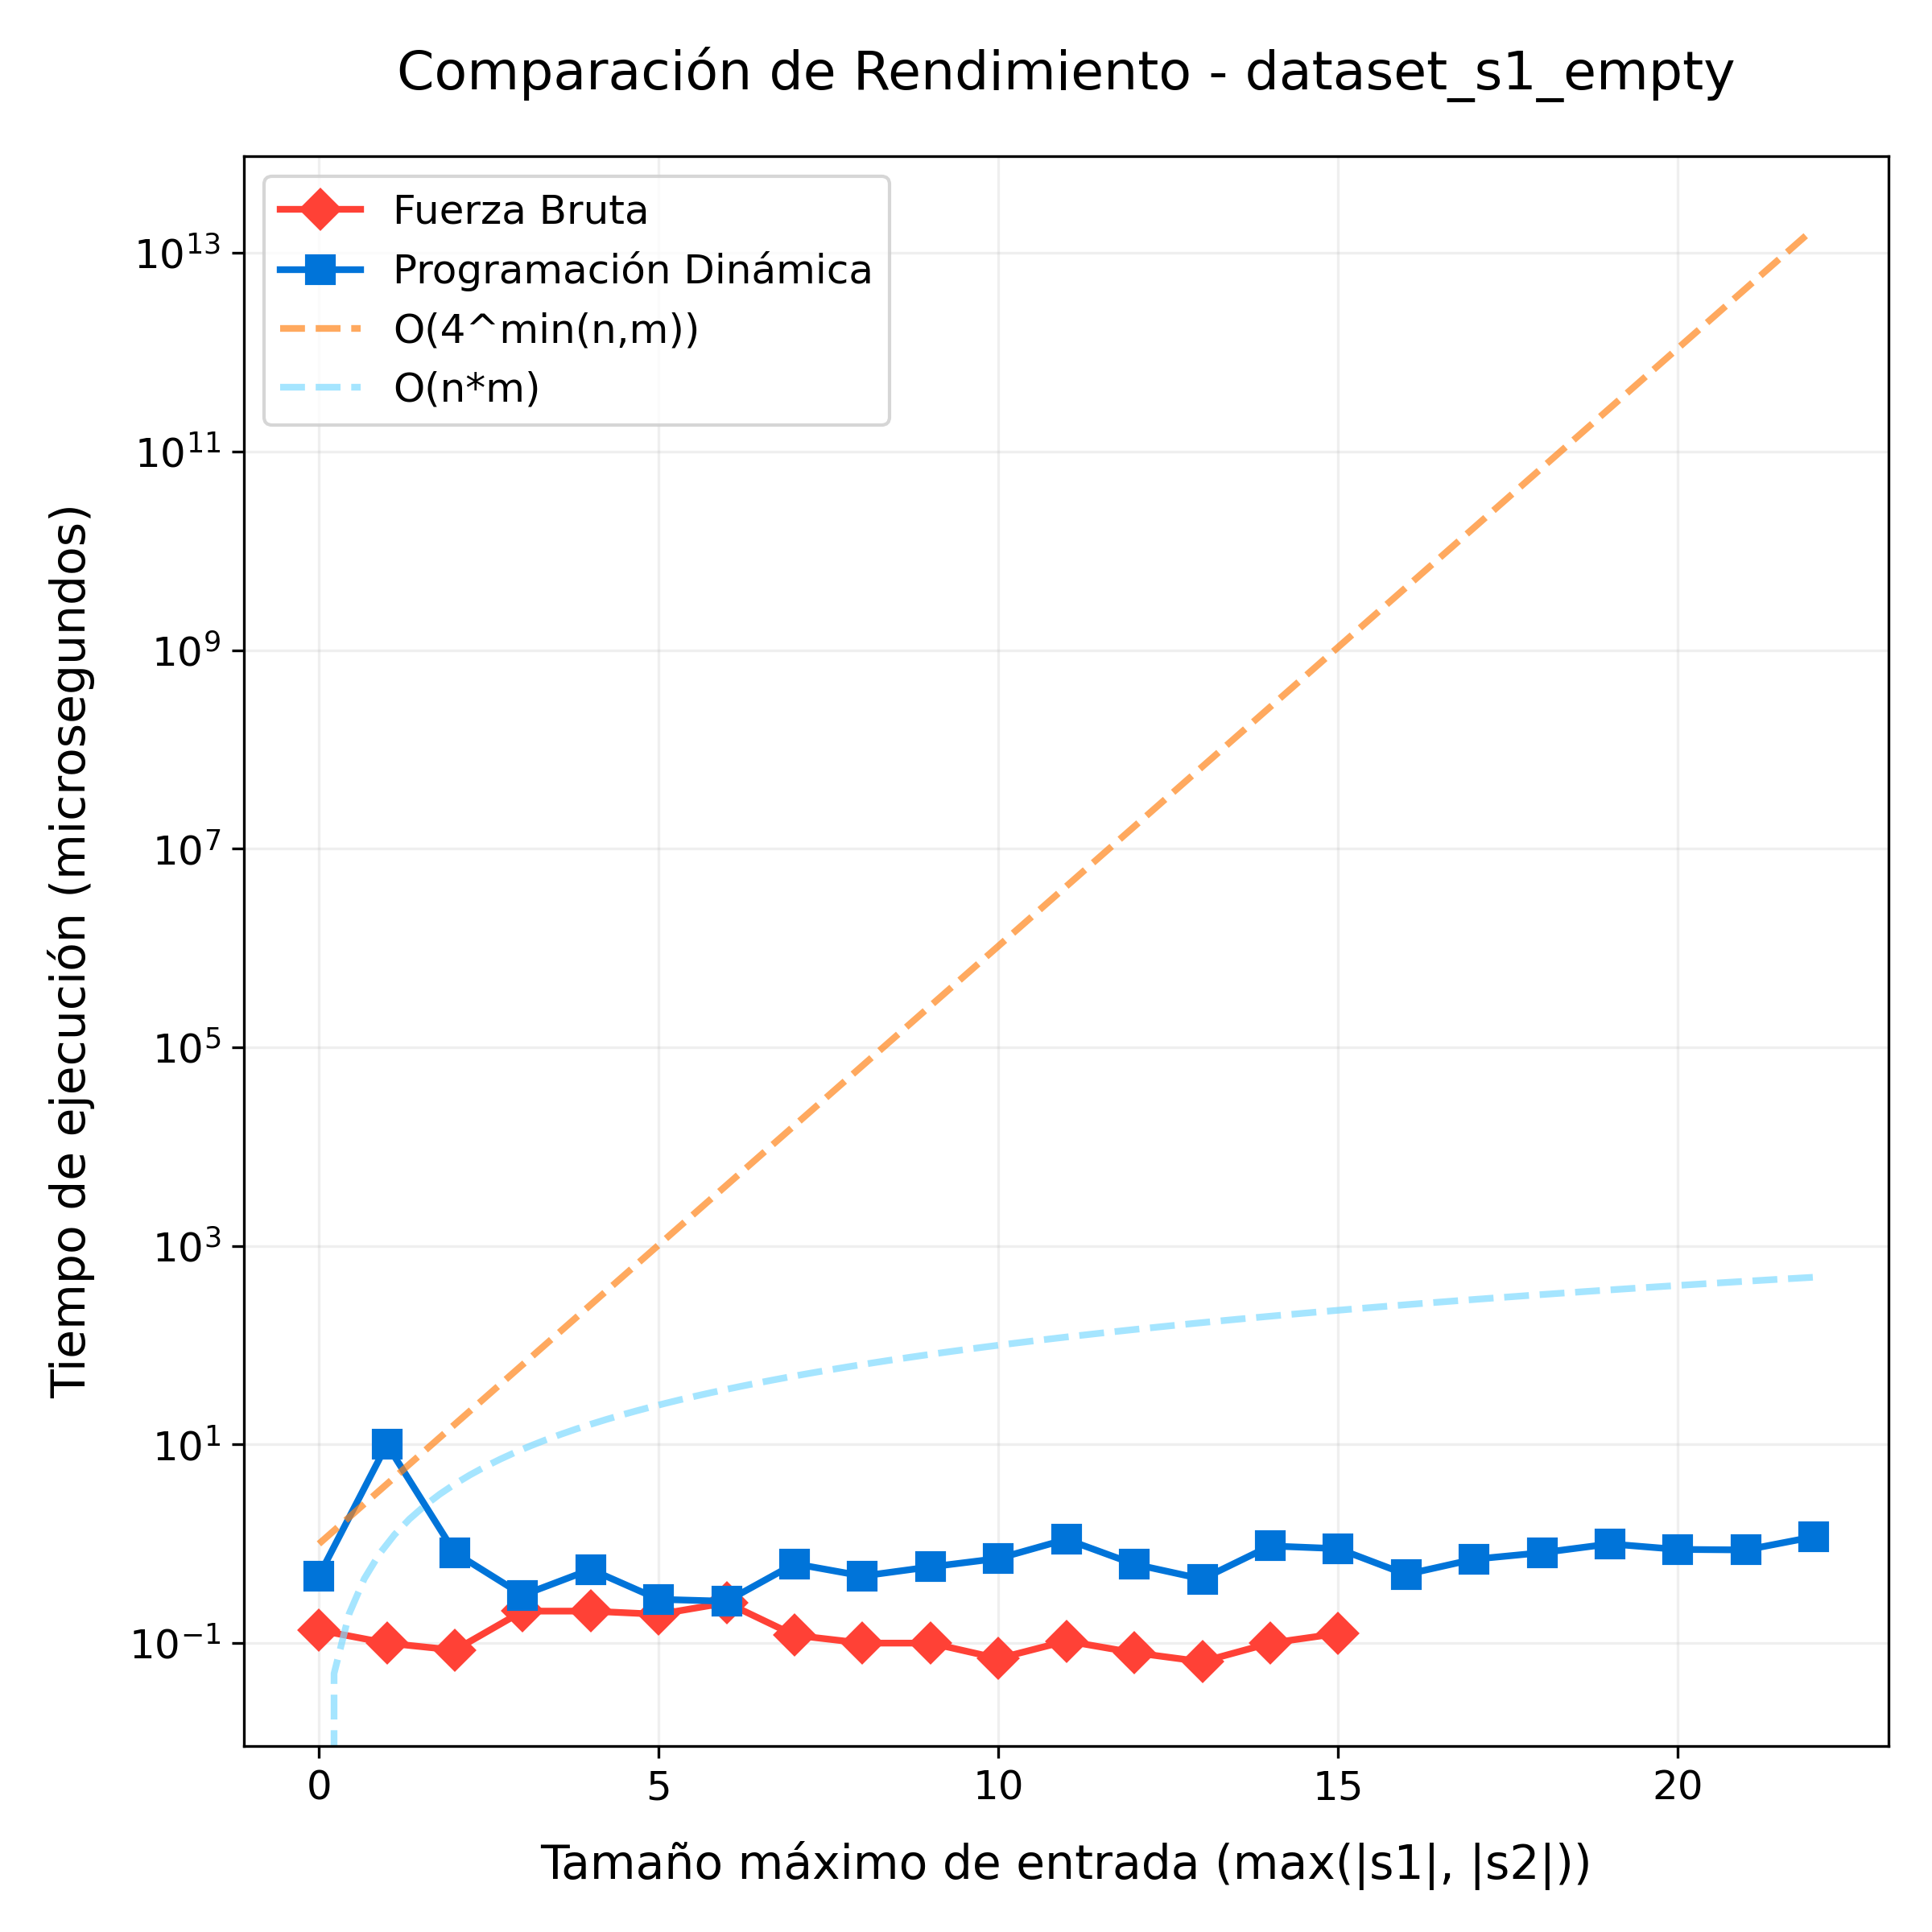
\includegraphics[width=\textwidth]{images/comparacion_dataset_s1_empty.png}
    \end{minipage}%
    \begin{minipage}[t]{0.5\textwidth}
        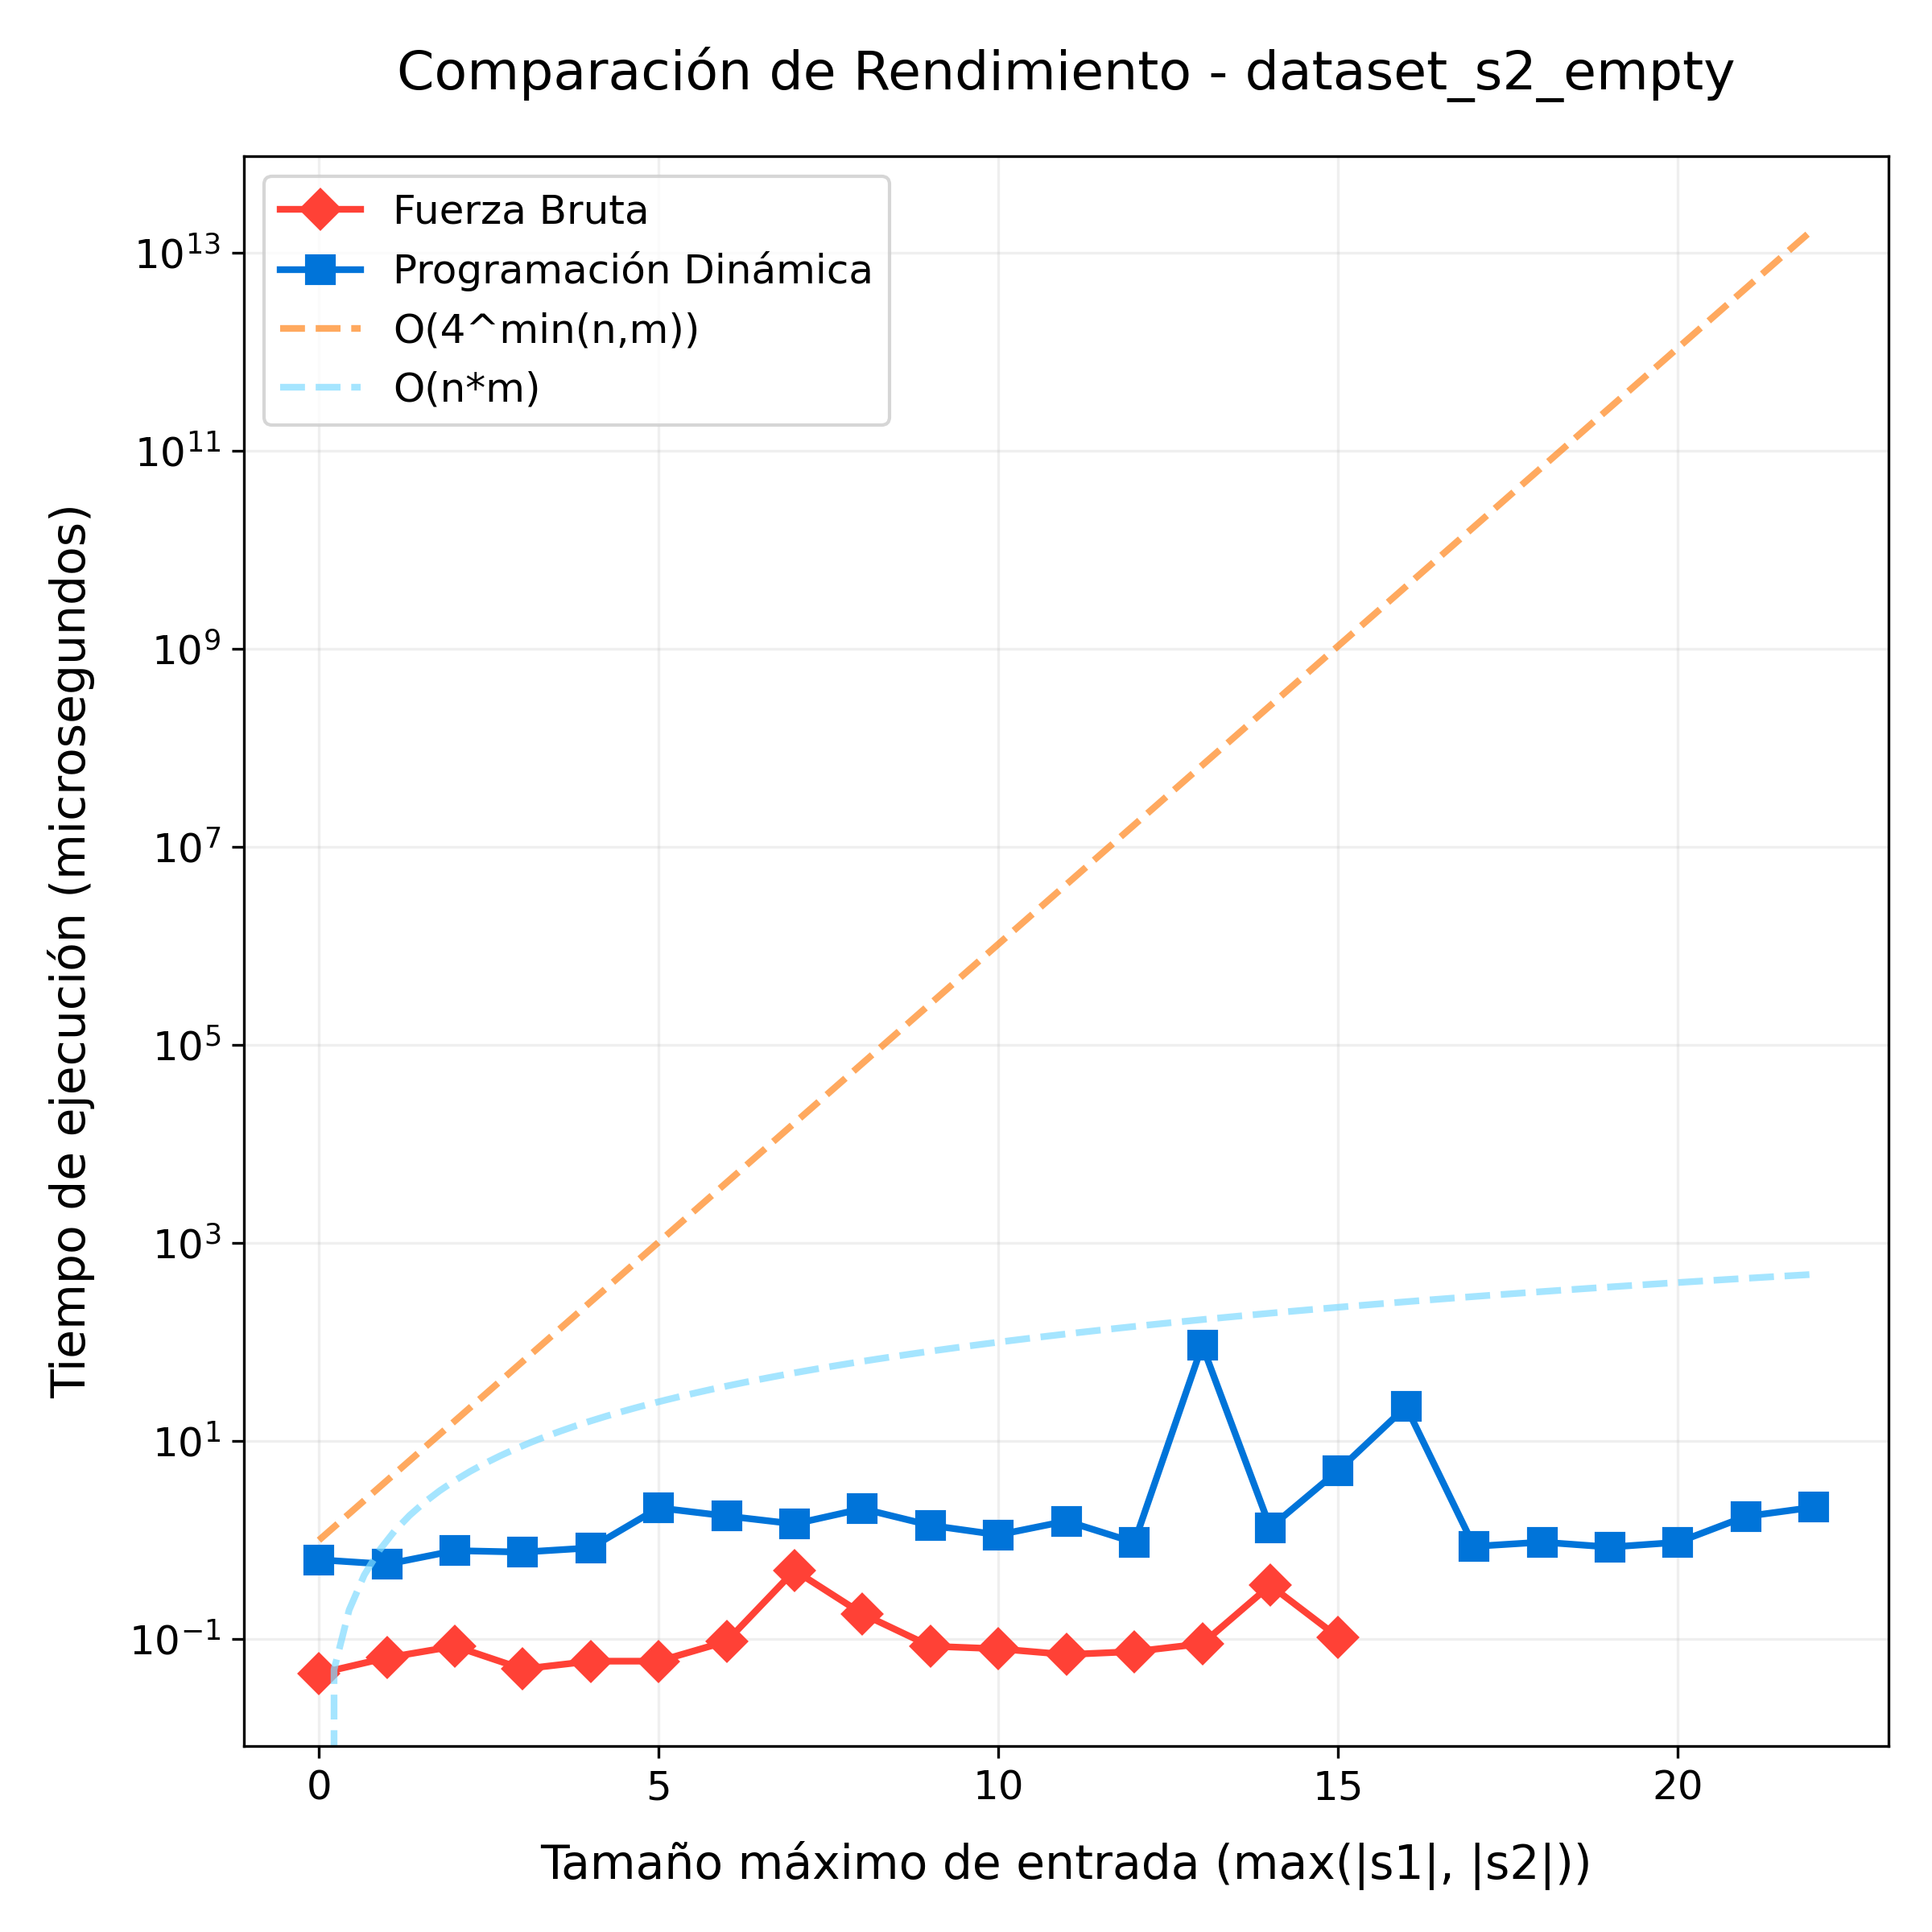
\includegraphics[width=\textwidth]{images/comparacion_dataset_s2_empty.png}   \end{minipage}%
    \caption{Comparación de rendimiento en datasets 1 y 2.}
    \label{fig:dataset1_2}
\end{figure}

En la Figura 1 podemos ver como, si bien el algoritmo DP presenta un coportamiento esperado en base a su complejidad temporal, 
su contraparte de BF se aleja considerablemente de la teoría. Esto, de hecho, lo esperábamos desde la definición del algoritmo, 
ya que para estos datasets nuestra solución cae constantemente en un caso base, realizando exclusivamente operaciones de adición hasta 
recorrer el string no vacío, superando así en rendimiento incluso al enfoque DP.  

\begin{figure}[H]
    \centering
    \begin{minipage}[t]{0.5\textwidth}
        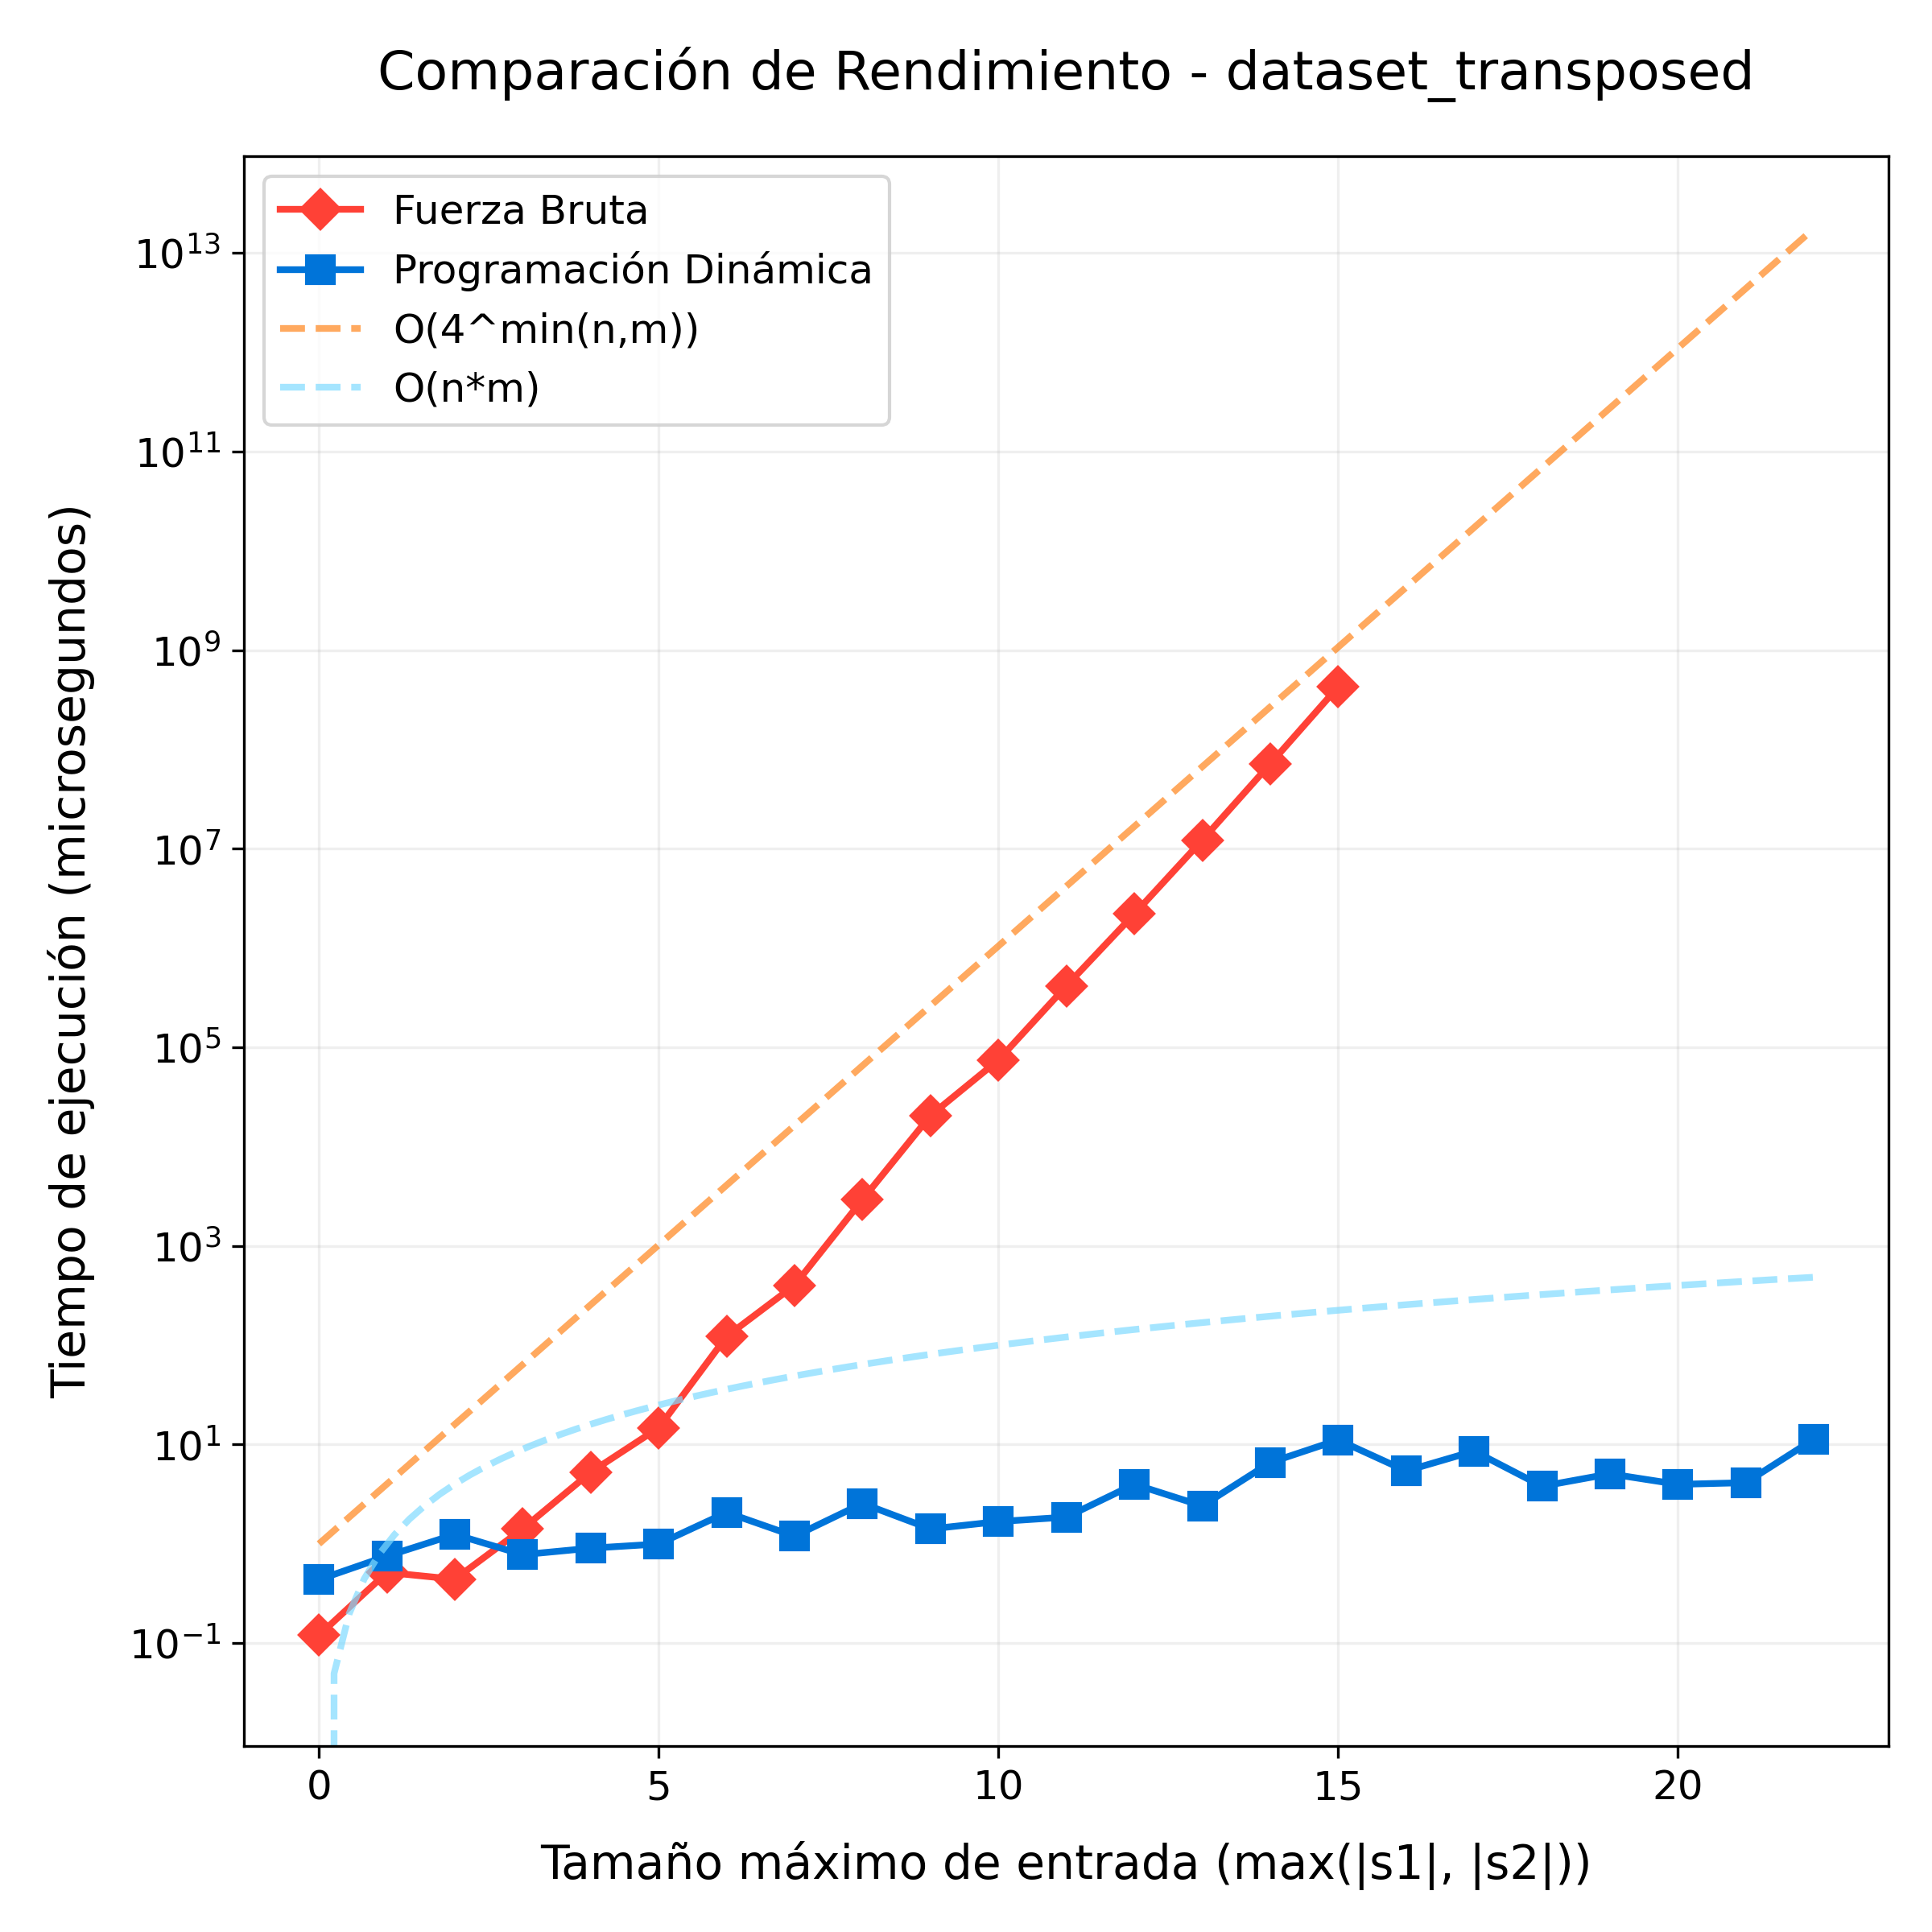
\includegraphics[width=\textwidth]{images/comparacion_dataset_transposed.png}   
    \end{minipage}%
    \begin{minipage}[t]{0.5\textwidth}
        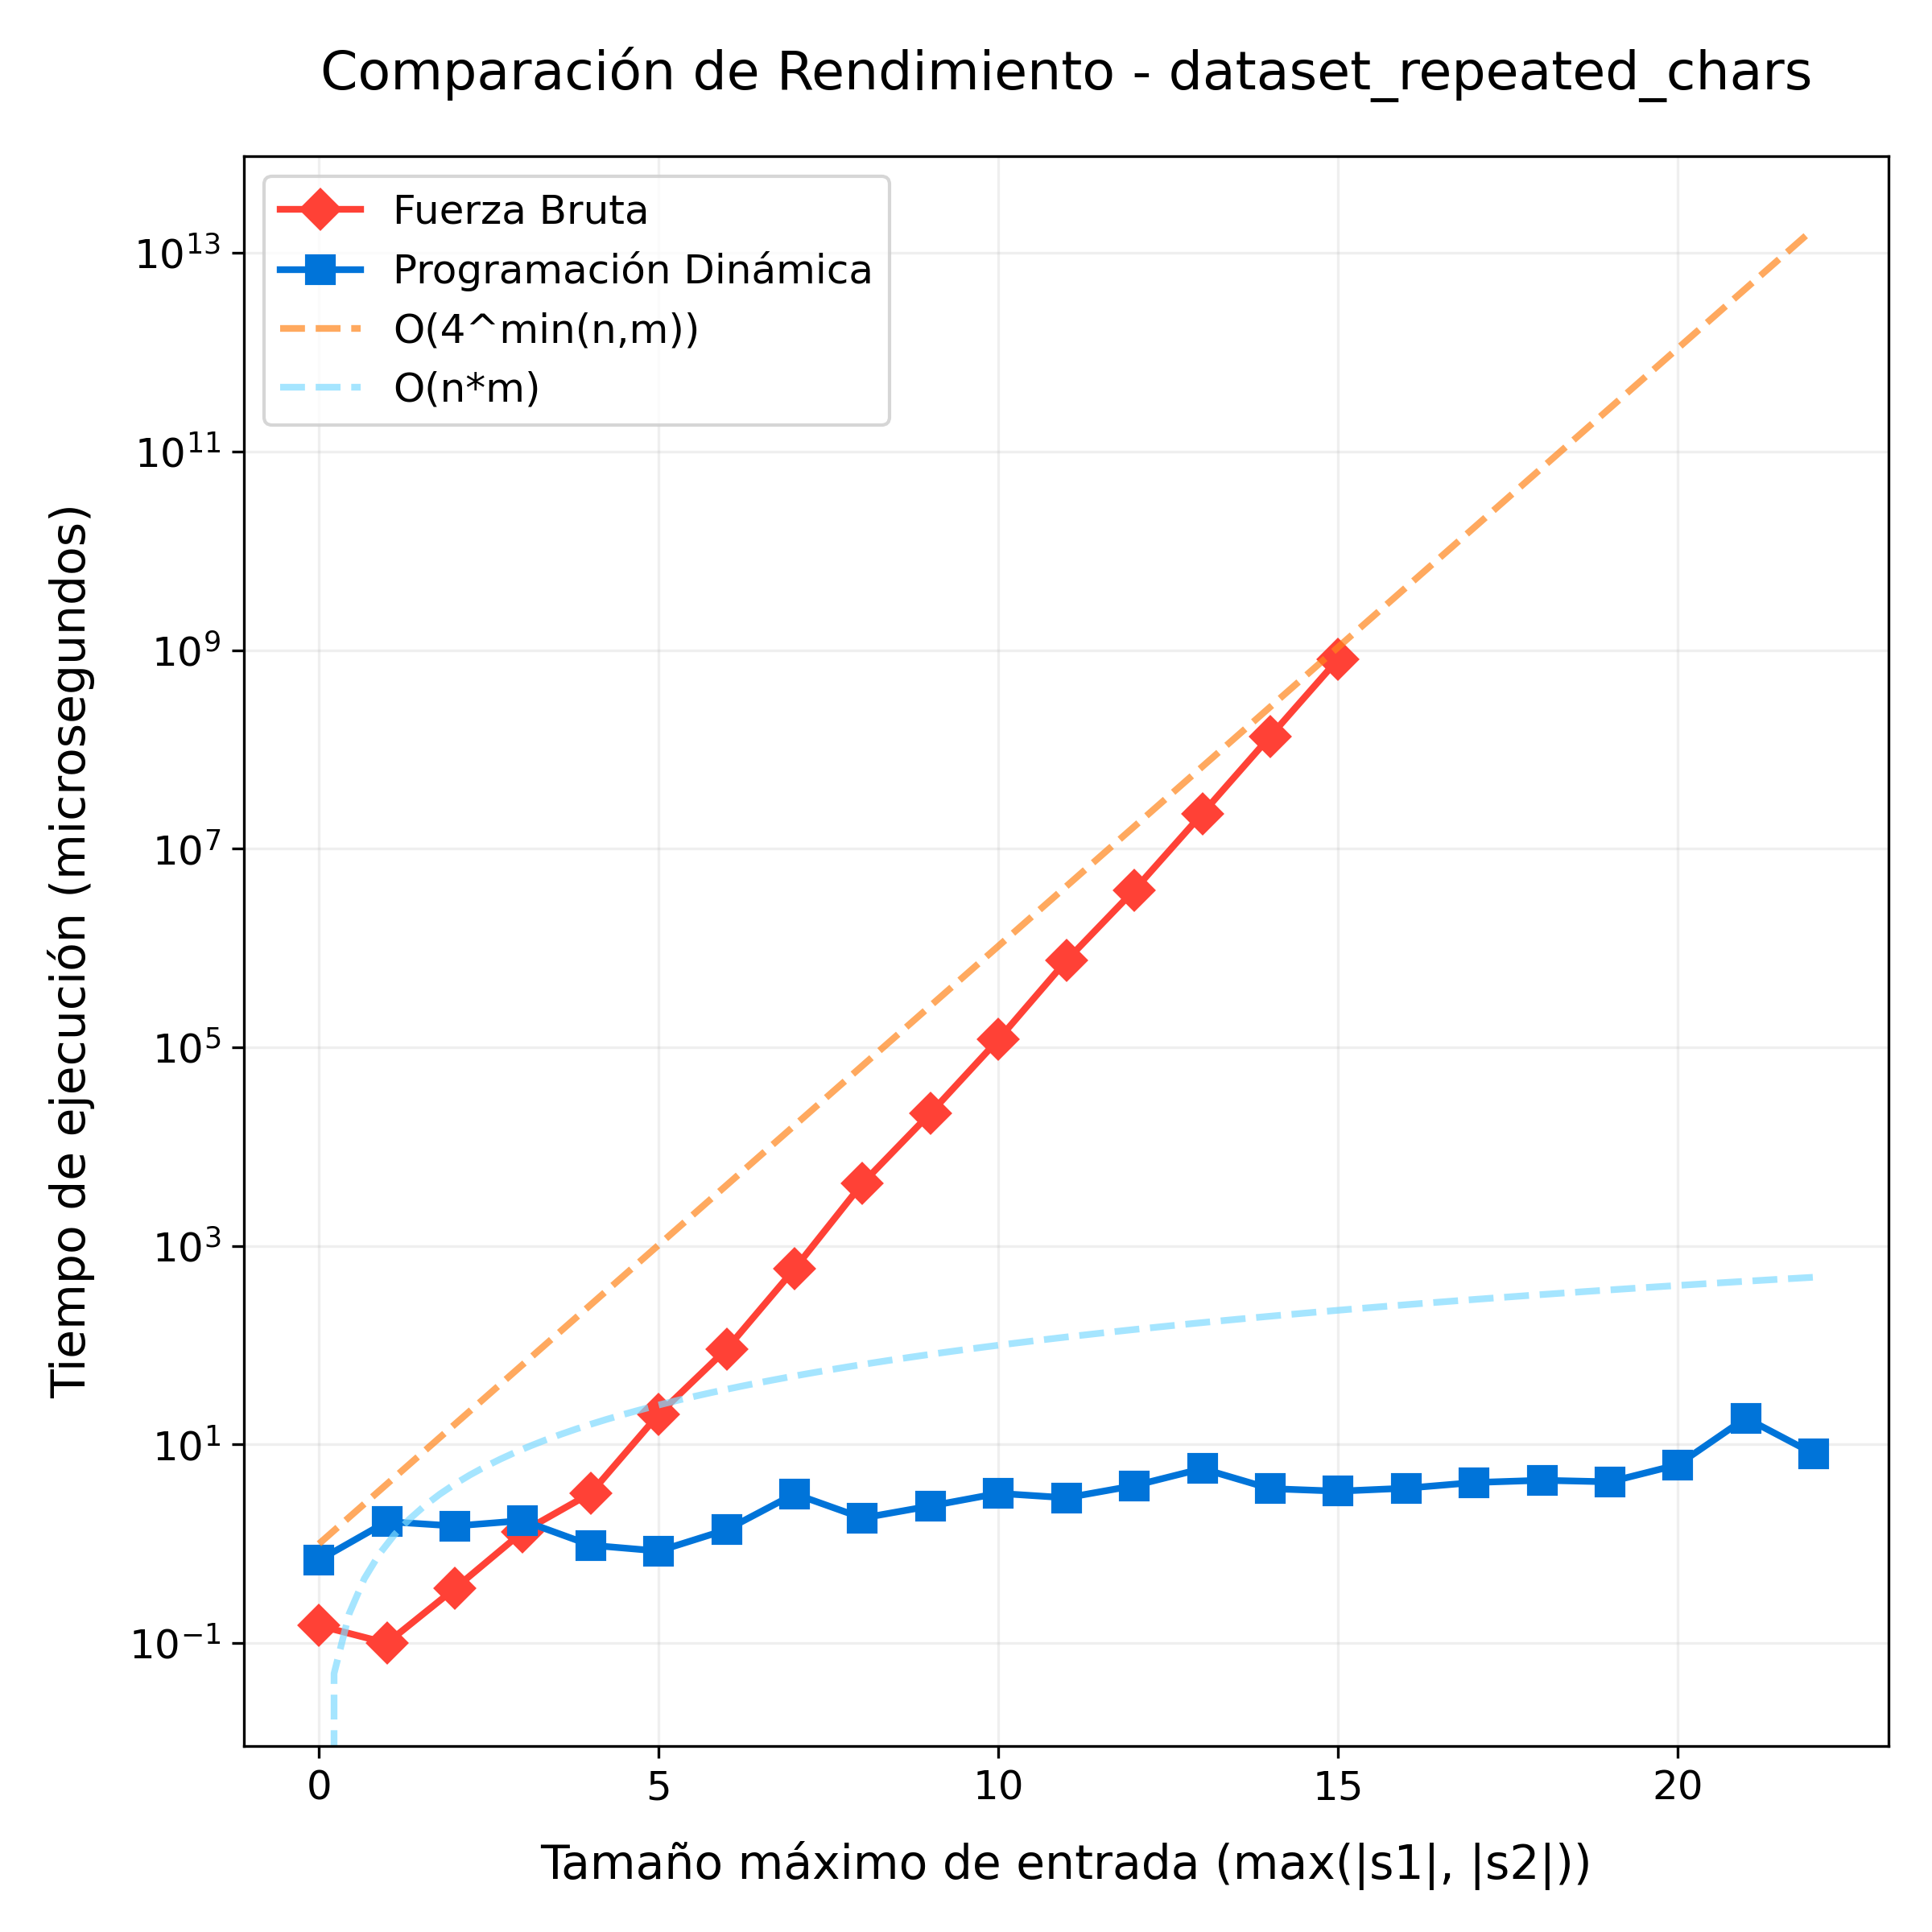
\includegraphics[width=\textwidth]{images/comparacion_dataset_repeated_chars.png} \end{minipage}%
    \caption{Comparación de rendimiento en datasets 3 y 4.}
    \label{fig:dataset3_4}
\end{figure}

En la Figura 2, vemos que DP no cambia, pero BF sufre las consecuencias de su complejidad exponencial, esta vez siguiendo la linea de tendencia esperada según el cálculo 
teórico planteado previamente.

\begin{figure}[H]
    \centering
    \begin{minipage}[t]{0.5\textwidth}
        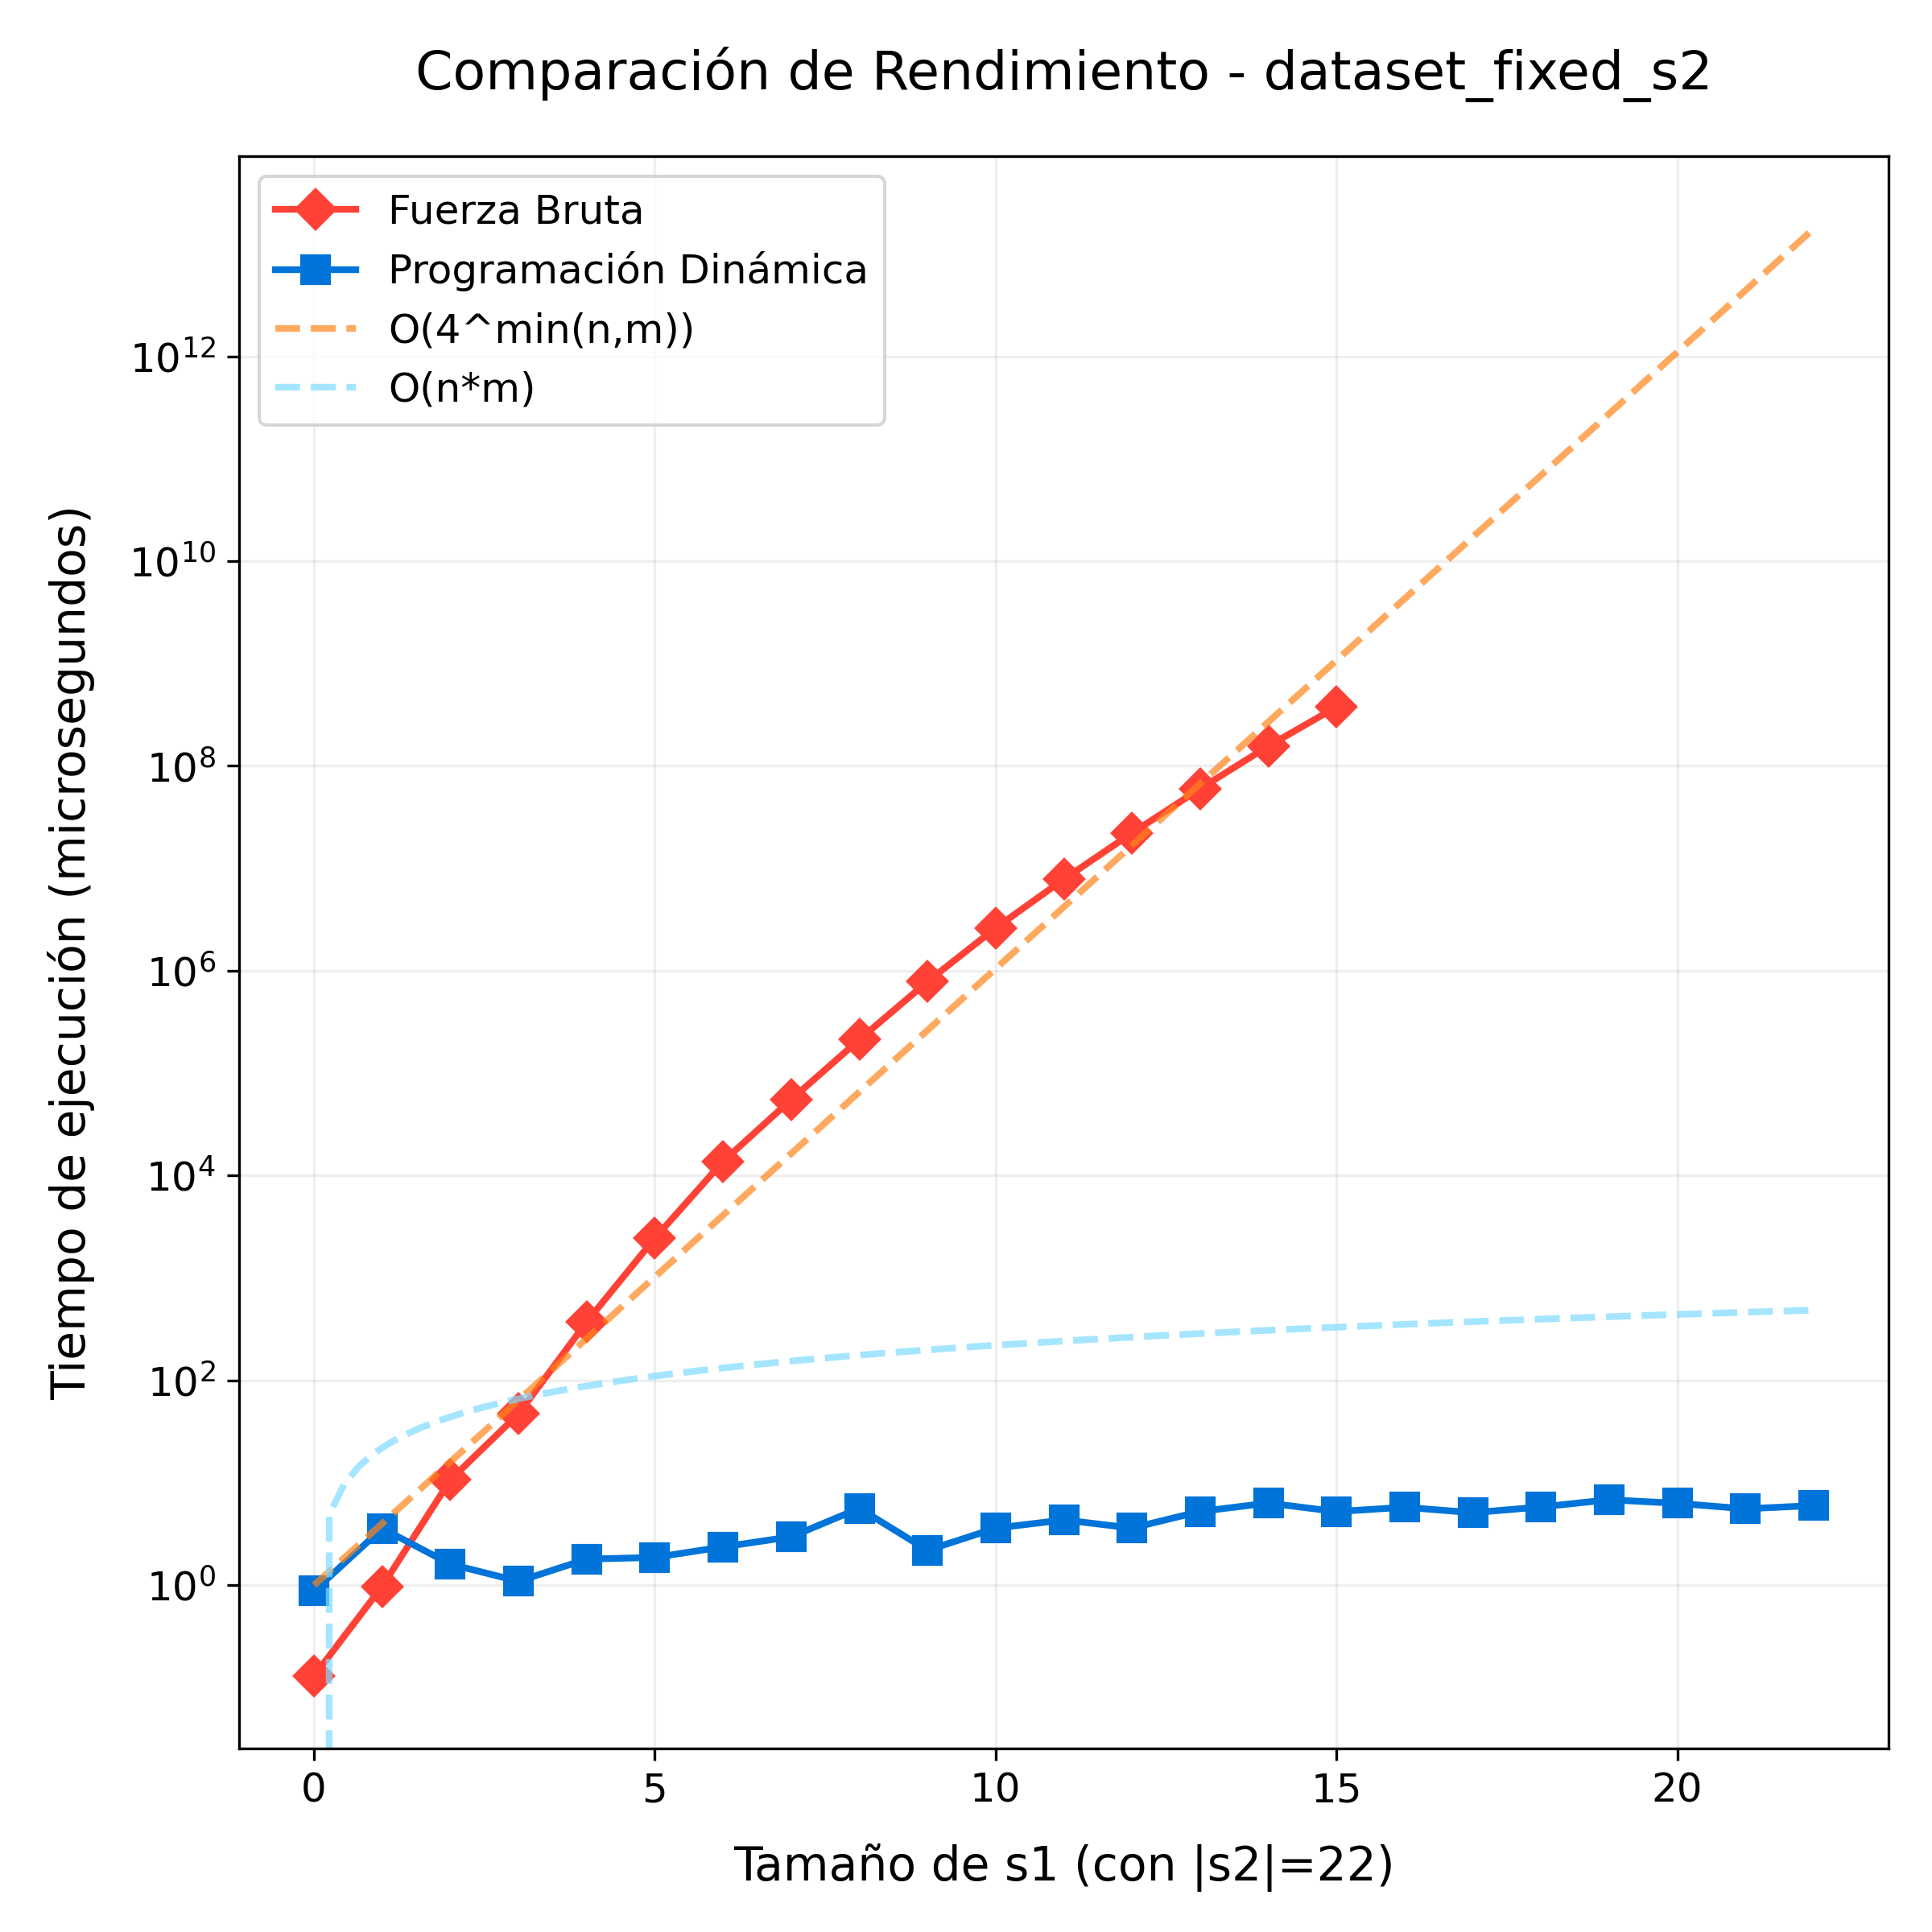
\includegraphics[width=\textwidth]{images/comparacion_dataset_fixed_s2.png}  
    \end{minipage}%
    \caption{Rendimiento dataset 5}
    \label{fig:dataset5_general_memoria}
\end{figure}

En la Figura 3 podemos ver nuevamente el comportamiento exponencial esperado de BF y como DP se mantiene bajo su curva de complejidad. 
Si nos fijamos, bajo este dataset, BF presenta un rendimiento aún peor que en los anteriores. Esto se debe a que s2, al ser constantemente de 
largo máximo, provoca que el tiempo de ejecución aumente con respecto a los largos variables de los datasets anteriores. 

\begin{figure}[H]
    \centering
        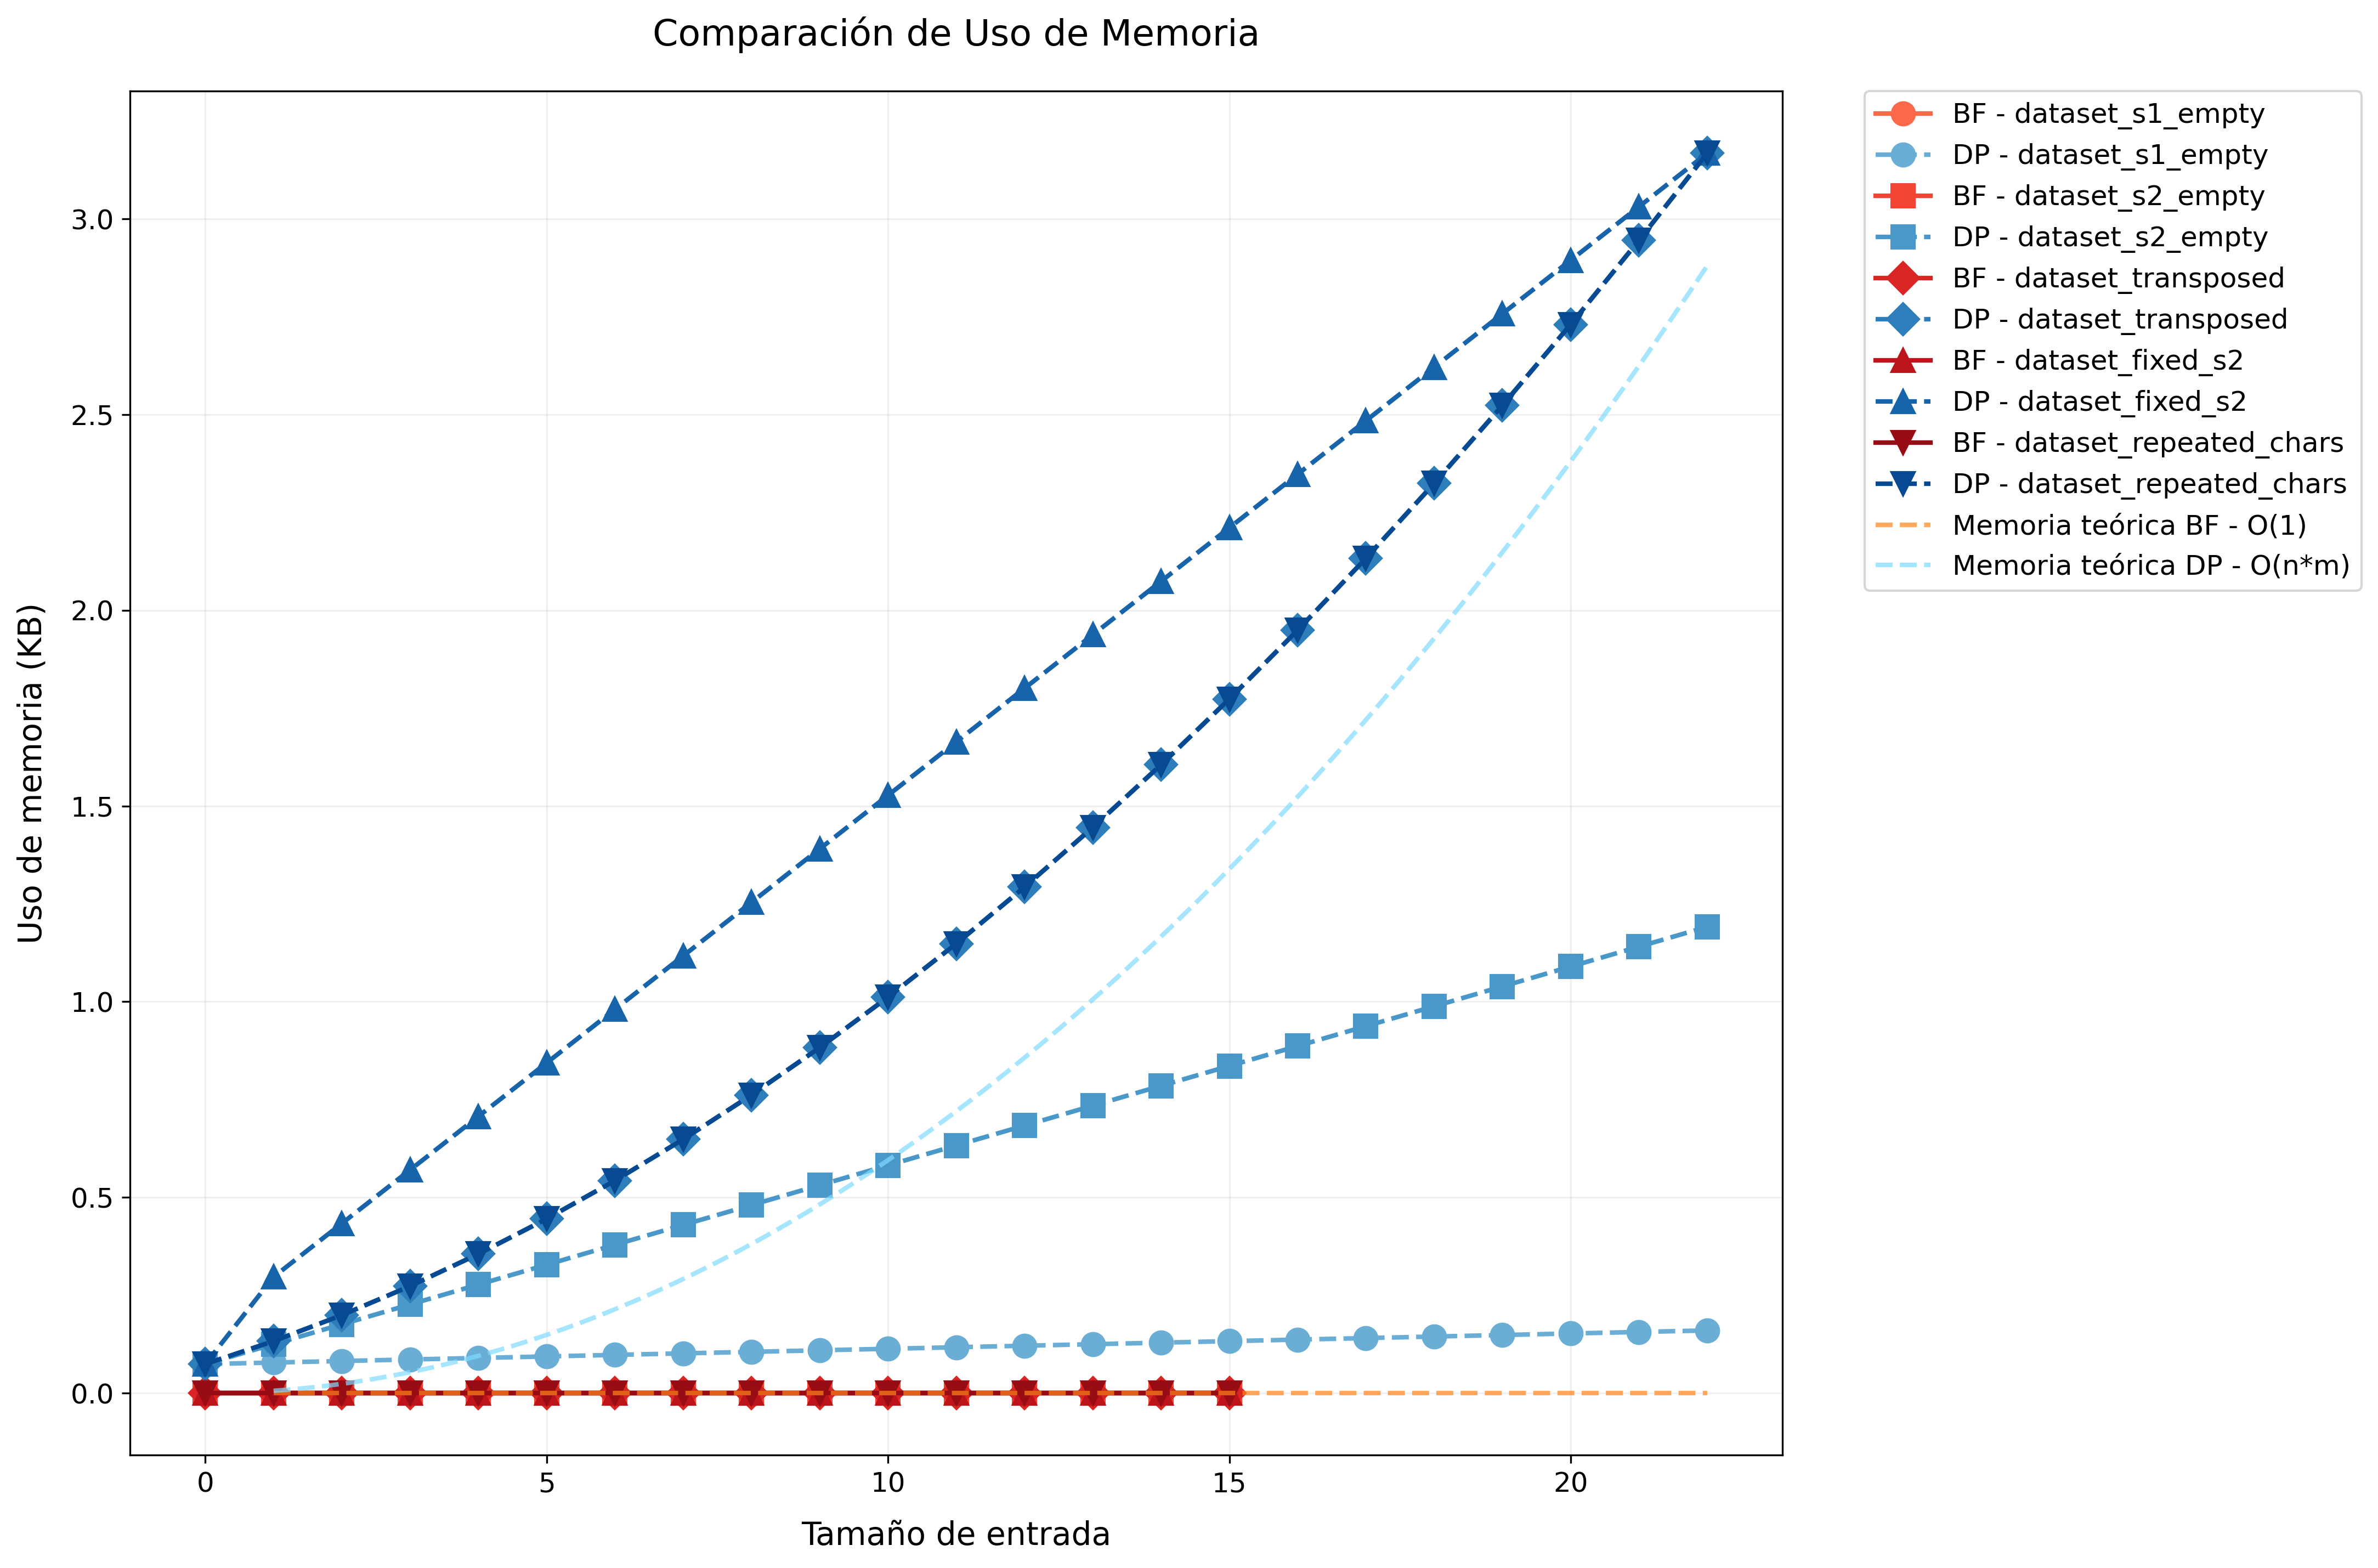
\includegraphics[width=\textwidth]{images/comparacion_memoria.png}
    \caption{Comparación general de uso de memoria}
    \label{fig:general_memoria}
\end{figure}

En la Figura 4 vemos un gráfico general del uso de memoria de cada algoritmo dependiendo del dataset. Podemos notar que para el primer dataset, 
DP ocupa una mínima cantidad de memoria, ya que solo tabula un arreglo. Las mediciones superiores muestran un coportamiento acorde a 
el cálculo teórico, presentando un crecimiento cuadrático. La medición más extravagante es la del dataset 2, es curioso ver que no se comporta como 
su contraparte de s1 vacío (dataset 1). Esto se debe a que para este caso, en vez de solo tabular un arreglo, DP tabula m arreglos de tamaño 1, 
eso explica la considerable diferencia con el dataset 1 pero que tampoco crece de manera cuadrática como el resto de casos. Por su parte, BF se mantiene 
nulo en el uso de memoria, ya que es un algoritmo in-place.

\begin{figure}[H]
    \centering
        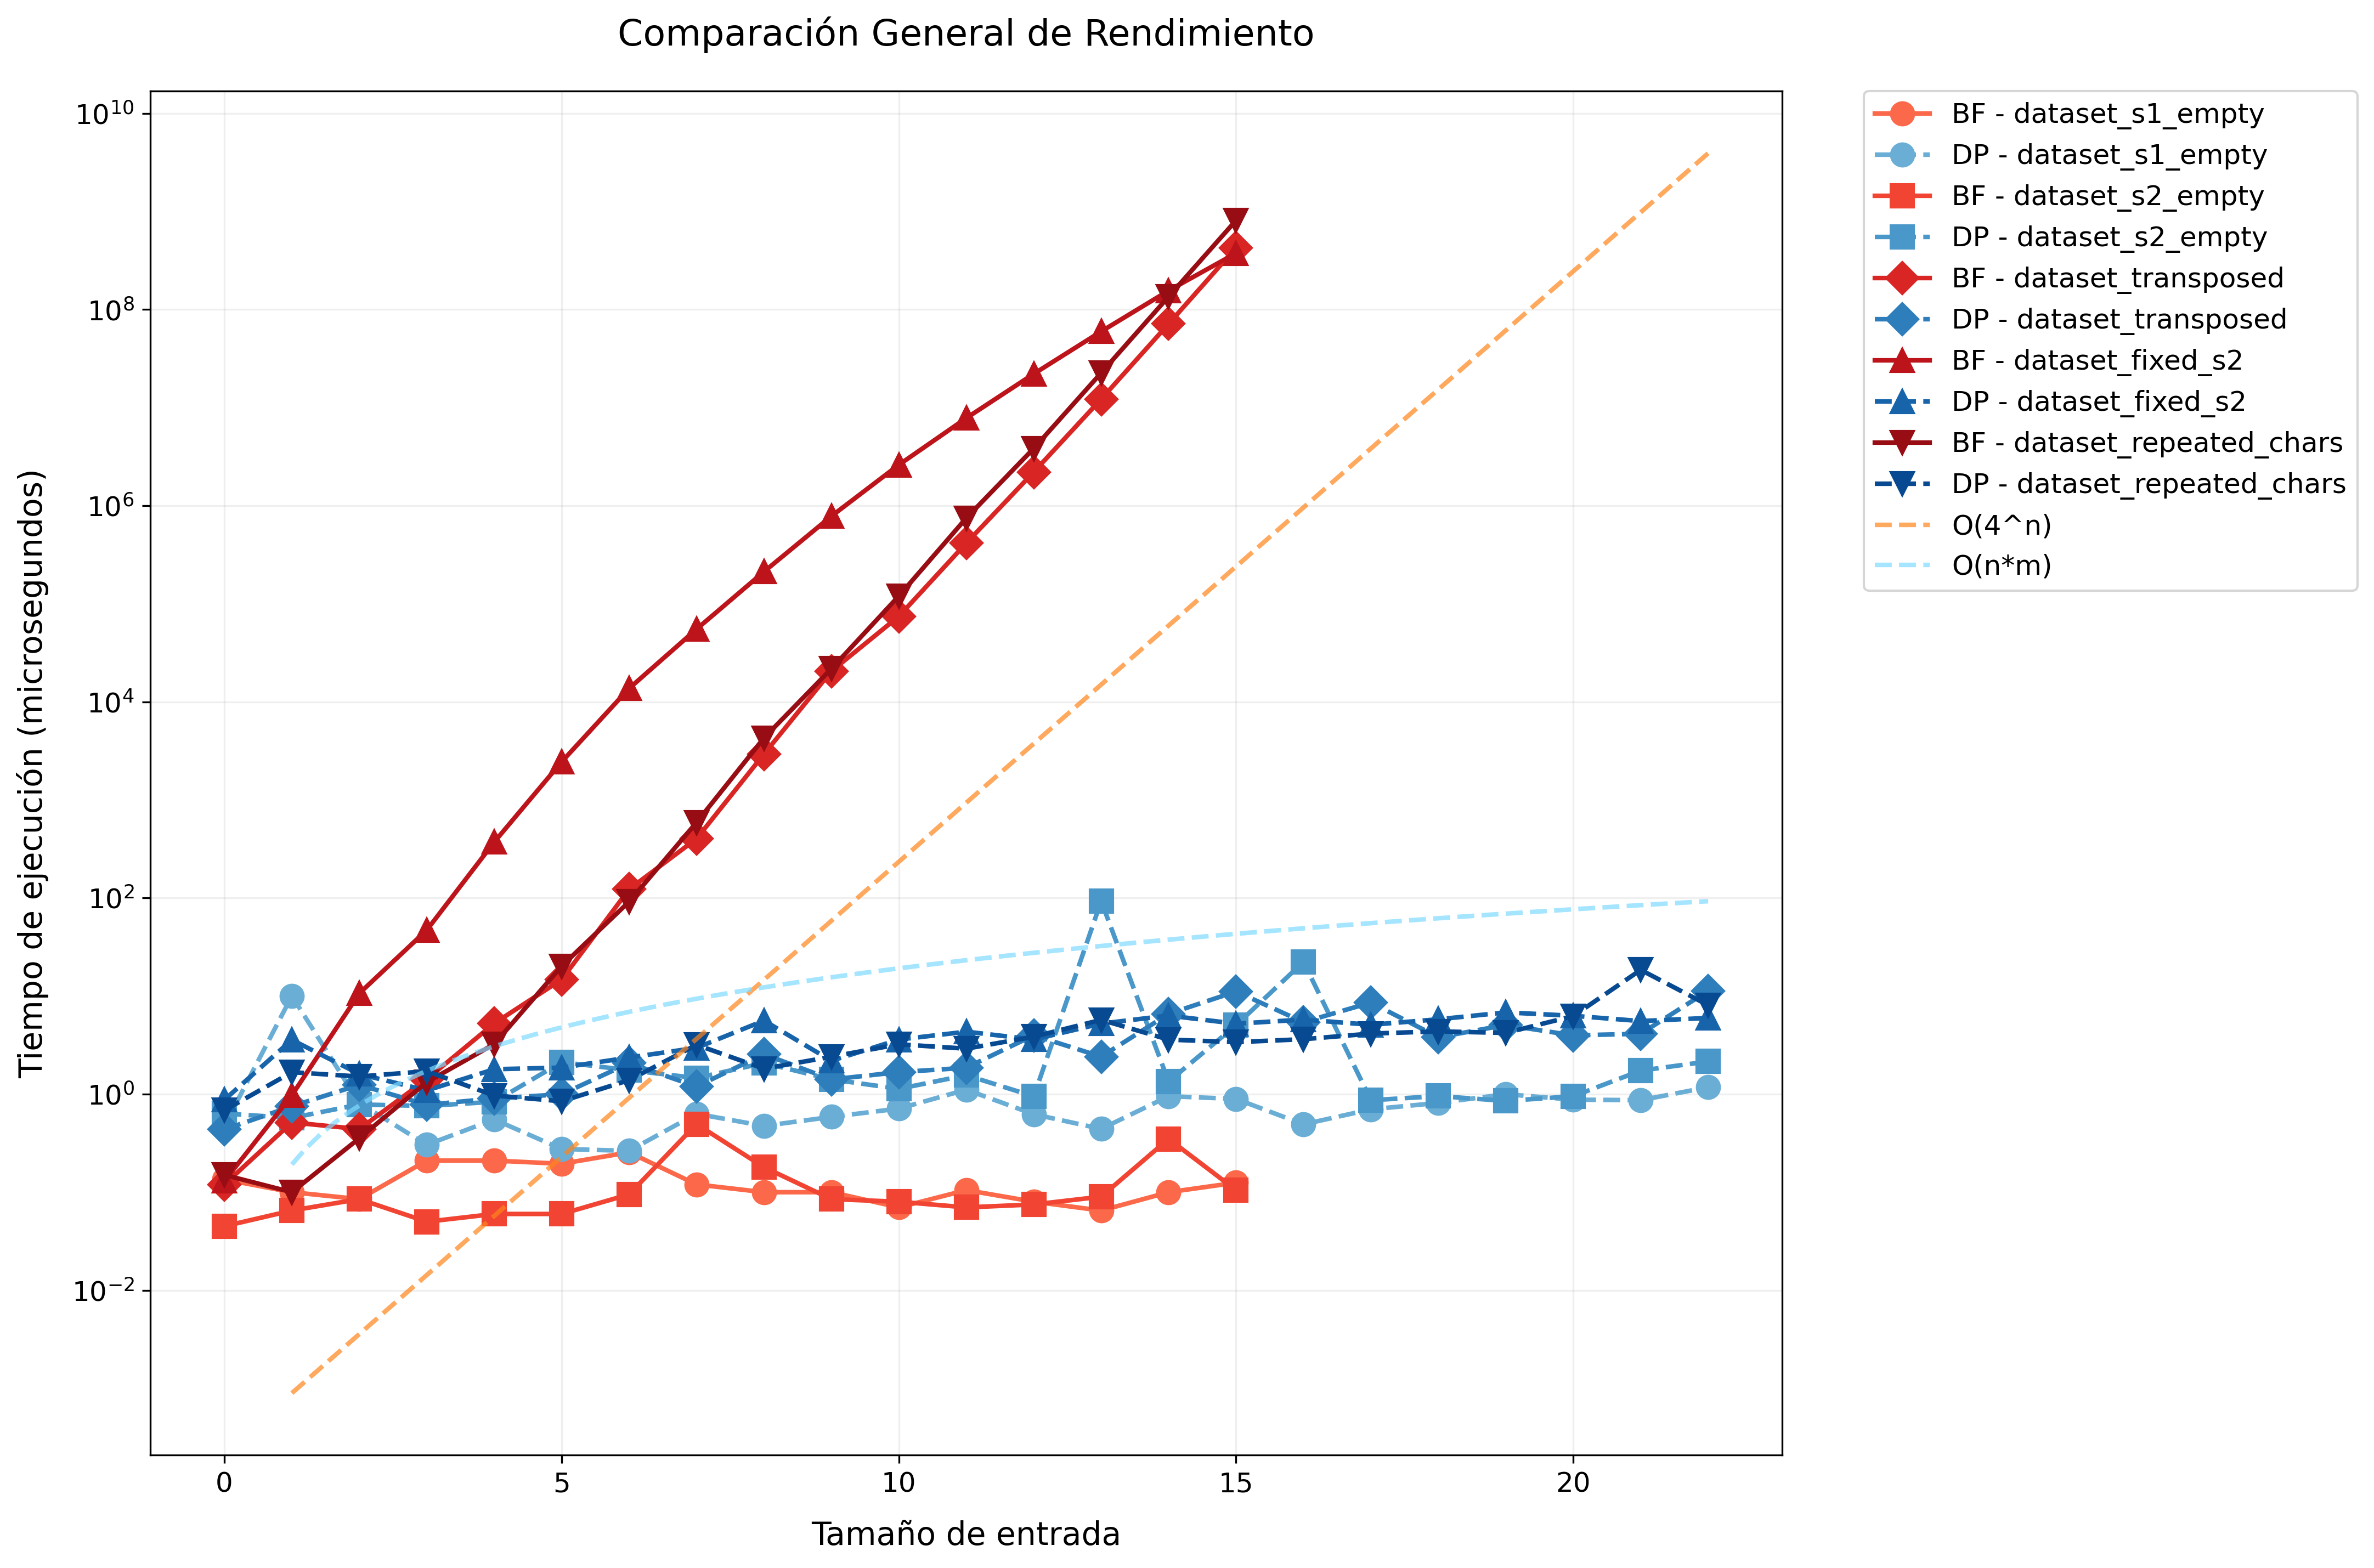
\includegraphics[width=\textwidth]{images/comparacion_general.png}   
    \caption{Comparación general de rendimiento}
    \label{fig:general}
\end{figure}

La Figura 5 presenta una comparación entre todas las mediciones de rendimiento vistas previamente. Podemos ver, como en los datasets 1 y 2, gracias a los casos base, BF 
presentan el mayor rendimiento de todos. Tambien, como en todas y cada una de las mediciones DP respeta su línea teórica, presentando un rendimiento excepcional que supera 
considerablemente las ejecuciones no particulares de BF. Para finalizar, se ve claramente como para los datasets 3, 4 y 5, BF tiene un crecimiento exponencial, siguiendo 
el ratio de la linea teórica, también podemos notar que nuestras predicciones de peor caso planteadas al diseñar el algoritmo eran correctas, ya que el peor tiempo de ejecución 
pertenece a BF en el \textbf{dataset 4 : repeated chars}, un dataset diseñado específicamente para permitir que en todas las llamadas del algoritmo se pueda considerar la opción de 
transponer, maximizando el número de llamadas recursivas, de esta forma logrando un peor rendimiento. 




